\documentclass[a4paper]{article}
\usepackage{interspeech2012,amssymb,amsmath,graphicx}
\sloppy	% better line breaks
%\ninept	% optional

\title{Identifying Speakers' Personal Information in Phone Conversations}

%%%%%%%%%%%%%%%%%%%%%%%%%%%%%%%%%%%%%%%%
%% If multiple authors, uncomment and edit the lines shown below.       %%
%% Note that each line must be emphasized {\em } by itself.                  %%
%% (by Stephen Martucci, author of spconf.sty).                                     %%
%%%%%%%%%%%%%%%%%%%%%%%%%%%%%%%%%%%%%%%%
%\makeatletter
%\def\name#1{\gdef\@name{#1\\}}
%\makeatother
%\name{{\em Firstname1 Lastname1, Firstname2 Lastname2, Firstname3 Lastname3,}\\
%      {\em Firstname4 Lastname4, Firstname5 Lastname5, Firstname6 Lastname6,
%      Firstname7 Lastname7}}
% End of required multiple authors changes %%%%%%%%%%%%%%%%%

\makeatletter
\def\name#1{\gdef\@name{#1\\}}
\makeatother
\name{{\em Shi Hu, Peter Lipay}}

\address{Stanford University \\
{\small \tt \{s3hu and plipay\}@cs.stanford.edu}}

%\twoauthors{Karen Sp\"{a}rck Jones.}{Department of Speech and Hearing \\
%  Brittania University, Ambridge, Voiceland \\
%  {\small \tt Karen@sh.brittania.edu} }
%  {Rose Tyler}{Department of Linguistics \\
%  University of Speechcity, Speechland \\
%  {\small \tt RTyler@ling.speech.edu} }

\begin{document}
\maketitle


\begin{abstract}
In this report, we investigate various methods to estimate a speaker's background information using their phone conversations and the corresponding transcripts. Among other results, we achieved 98\% estimation accuracy in gender, and 68\% in education level using speech data alone. This report also includes the most discriminative words for gender derived from the KL distance, and a simulation of a speech recognition system to show the robustness of our methods using the ``transcribed'' text.
\end{abstract}


\section{Introduction}
Being able to automatically identify a speaker's background information in a phone conversation can have many benefits. For example, when a human interacts with a conversational agent, knowing the person's age can help machines customize their responses. Other usages may include targeted advertising and criminal investigation. In this report, we estimate a speaker's age, gender, education level and American English accent using their speech and transcripts in phone conversations.

\section{Related Work}
Bahari et al. extracted speech patterns based on i-vectors \cite{dehak}, then apply Support Vector Regression (SVR) to estimate the age of speakers \cite{bahari}. An i-vector or identity vector is a low-dimensional representation of a speaker obtained by projecting the speaker utterance onto the total variability space, which contains both speaker and channel variability (the basis is denoted as T in equation \ref{ivector}).  The speaker- and channel-dependent GMM mean supervector $\mu$ is modeled as:  
\begin{equation}
\mu = m + Tw
\label{ivector}
\end{equation}

Here, $m$ is the speaker- and channel-independent mean supervector. The i-vector is represented as $w$.

Bahari et al. used a 60 dimensional feature vector consisting of 20 MFCCs appended by the first and second order derivatives to train the GMM system, and used a variation of $\mu$ and $m$ to obtain the i-vector. They showed that the age is best estimated without any dimension reduction on the i-vector, and the mean absolute error (MAE) in years for male and female speakers' age is 7.63 and 7.61, respectively.

Garera and Yarowsky discussed several techniques to classify gender, age, etc using text only \cite{garera}. They used unigrams and bigrams with top tf-idf scores and stopwords as the features, and a linear SVM classifier for training and testing. For gender/age detection, they found the partner of a conversation has strong influence on the choice of words on both sides. Thus, they classify both partners jointly, e.g., male-male vs rest or female-female vs rest, and achieved better accuracy than classifying each partner separately. In addition, they found sociolinguistic features such as speaker rate and pronoun usage are good indicators of gender, etc.

Boulis and Ostendorf analyzed the differences in word use between genders using phone conversation transcripts \cite{boulis}. To obtain the best classification accuracy of conversation sides according to the genders, they used the top 70\% of all bigrams in the corpus as features, sorted by the KL distance, the tf-idf as the feature scores and SVM as the classifier. This achieved an accuracy of around 93\%. However, using only 3\% of the top bigrams can still achieve around 90\% accuracy. Further, they found the conversation partners influence each other's linguistic patterns; hence, it is easier to classify same-gender conversations than cross-gender. 

\section{Methods}

\subsection{Datasets}
We are using the Switchboard Phase 2 corpus which was recorded in 1991/2. There are 543 speakers and 2262 phone conversations, consisting of 243 hours of speaking time, and 2.9M spoken words. We want to separate out the two speakers in each conversation. For audio files, we used sox to extract the conversation side for each speaker, and concatenate all segments together. For text files, we extract and concatenate the utterences by speakers.

As for the speaker properties, there are 2 genders, 5 education levels, 10 American English accents and 6 age groups (grouped by decades). Their distributions are plotted in Figure \ref{dists}. For age, we also used regression to compute mean absolute error (MAE) using chronological age.

\begin{figure}[t]
\centerline{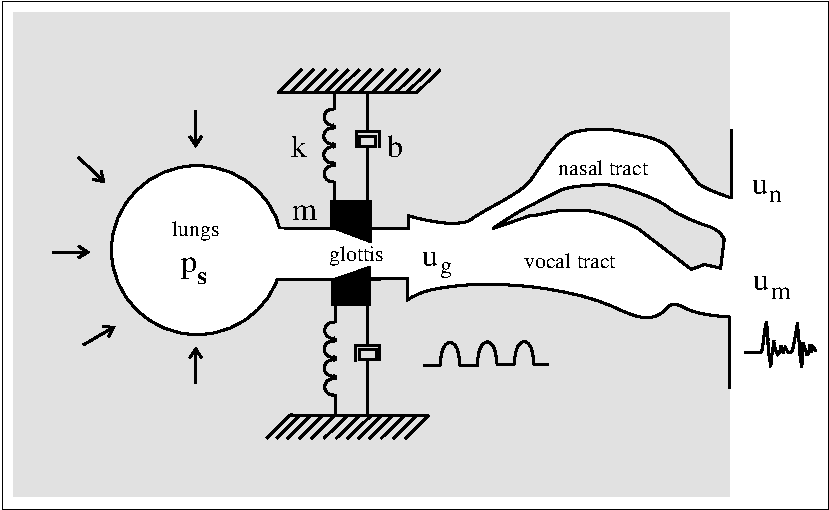
\includegraphics[width=80mm]{figure}}
\caption{{\it Speaker property distributions}}  
\label{dists}
\end{figure}

\subsection{Feature Selection}
\subsubsection{Audio}
We have tried three different types of features for audio, namely, openSMILE, MFCC and openSMILE+MFCC. We used the same feature for each property estimation.

\begin{itemize}
\item openSMILE \cite{eyben}: there are 384 features including the characteristics for the signal energy, MFCC and F0, etc. We think these are useful to identify gender and age, etc.
\item MFCC: we used Kaldi to extract MFCC
\item openSMILE+MFCC:
\end{itemize}

\subsubsection{Text}

\subsection{Classifiers}

\section{Experiments}
\subsection{Experimental Setup and Implementation Details}
\subsection{Audio}
\subsubsection{Features}
\subsubsection{Classifiers}

\subsection{Text}
\subsubsection{Features}
\subsubsection{Classifiers}
\subsubsection{Most Discriminative Words for Gender}
\subsubsection{Speech Recognition System Simulation}

\subsection{Audio + Text}

\section{Conclusions}

\section{Acknowledgements}

\eightpt
\bibliographystyle{IEEEtran}
\begin{thebibliography}{10}
\bibitem[1]{bahari} Bahari, M. H., et al., 
``Age Estimation from Telephone Speech using i-vectors'', 
Interspeech, 2012.

\bibitem[2]{dehak} Dehak, N., et al., 
``Front-End Factor Analysis for Speaker Verification'', 
IEEE Trans. Audio, Speech and Language Processing, 2011.

\bibitem[3]{garera} Garera, N. and Yarowsky D.,
``Modeling Latent Biographic Attributes in Conversational Genres'',
ACL/IJCNLP, 2009

\bibitem[4]{boulis} Boulis, B and Ostendorf, M.,
``A Quantitative Analysis of Lexical Differences Between Genders in Telephone Conversations'',
ACL, 2005

\bibitem[5]{eyben} Eyben F., Wöllmer. M. and Schuller, B.,
``openSMILE – The Munich Versatile and Fast Open-Source Audio Feature Extractor'',
ACM Multimedia, 2010

\bibitem[6]{povey} Povey D., et al.,
``The Kaldi Speech Recognition Toolkit''.

\end{thebibliography}
\end{document}
